\newpage
\section{Appendix}


\subsection{Full Hungarian Algorithm}
\label{FullHA}

As already mentioned in section \ref{SimpleTSP} of this article, the full Hungarian Algorithm takes an immense amount of time for any TSP of a reasonable scale. However, with a small problem like the one described in that section, it is not too problematic. What follows in this section is a full solution of the 6-city problem via the modified Hungarian Algorithm. 

\vspace{4mm}
\noindent Begin with the distance matrix:

\begin{center}
	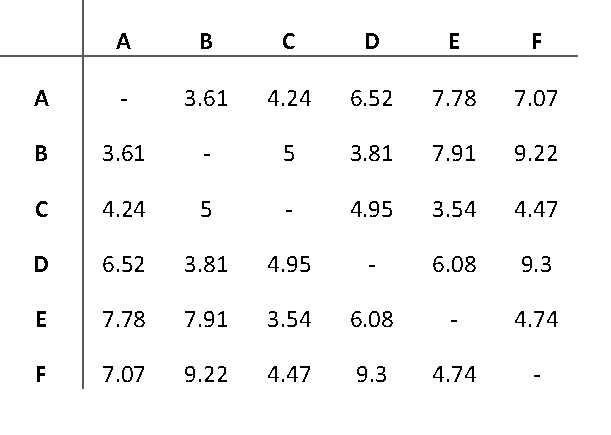
\includegraphics[height=5cm]{distancematrix}
\end{center}

\noindent
Perform the first step: row and column reduction. For that, subtract the smallest element of each row from its respective row, then do the same for columns, like so:

\begin{center}
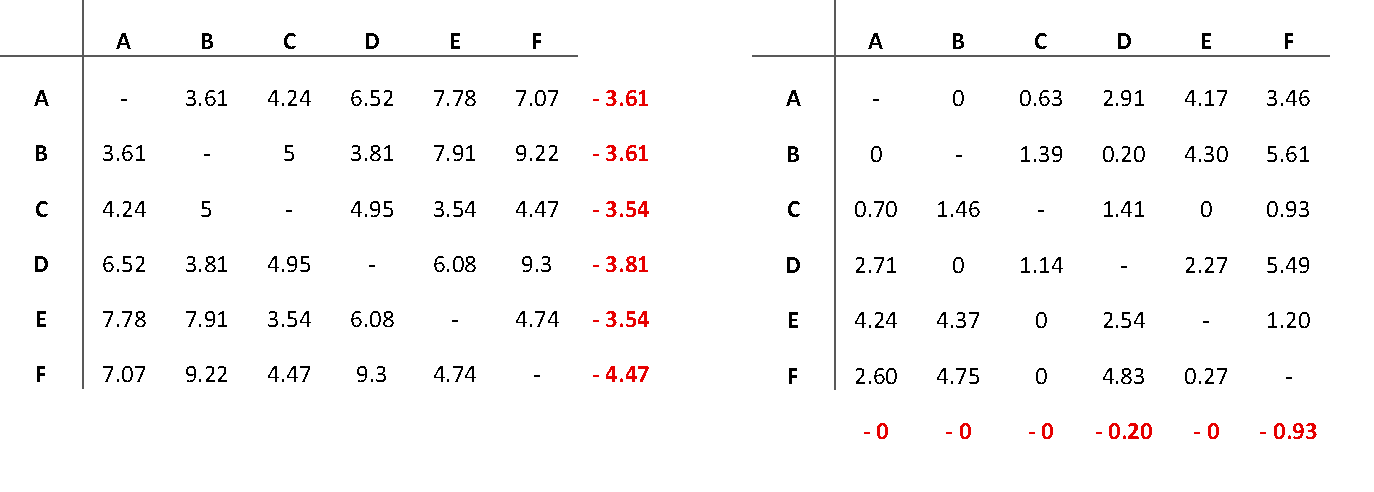
\includegraphics[height=5.2cm]{1red0}  
\end{center}

\noindent
This results in the following matrix, called the reduced distance matrix:

\begin{center}
	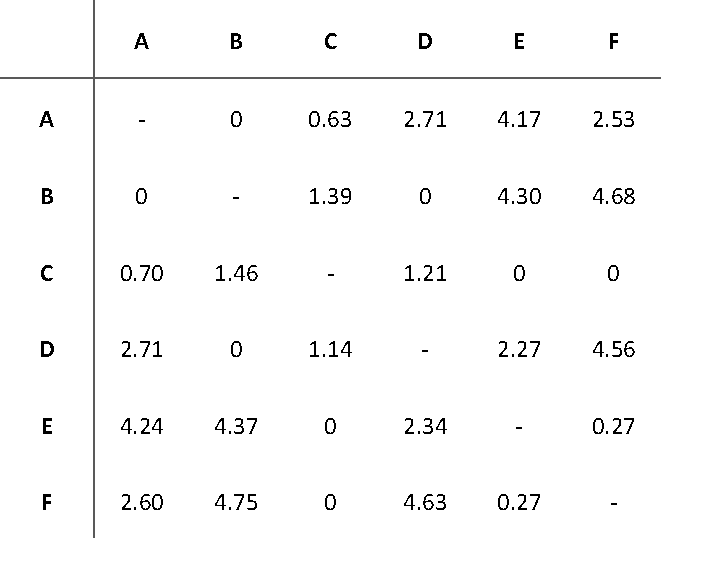
\includegraphics[height=6cm]{1red}
\end{center}
	
\noindent
The second step of the algorithm is penalty calculation. The penalty of a zero is the sum between the smallest element in the row and the smallest element in the column in which that zero stands. The figure below shows these penalties:

\begin{center}
	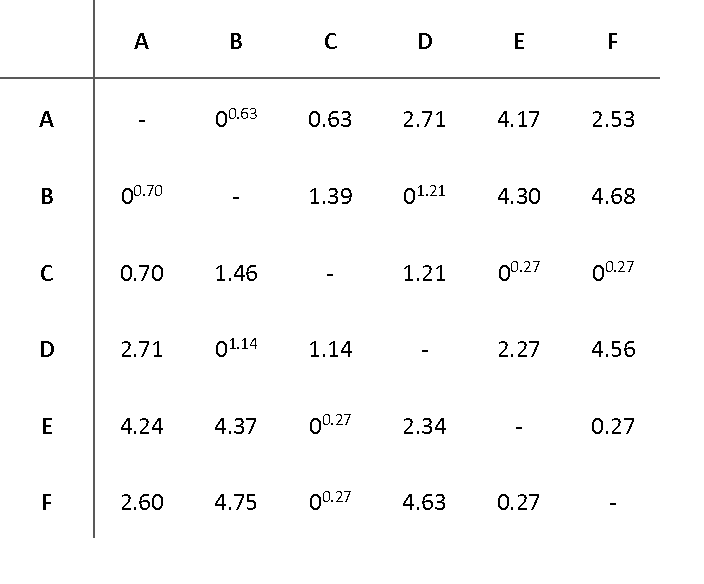
\includegraphics[height=6cm]{1pen}
\end{center}

\noindent
Third step is elimination. The row and the column of the zero with the highest penalty get eliminated from the matrix, leaving behind a smaller matrix and a fraction of the final tour. Hence, row B and column D get eliminated:

\begin{center}
	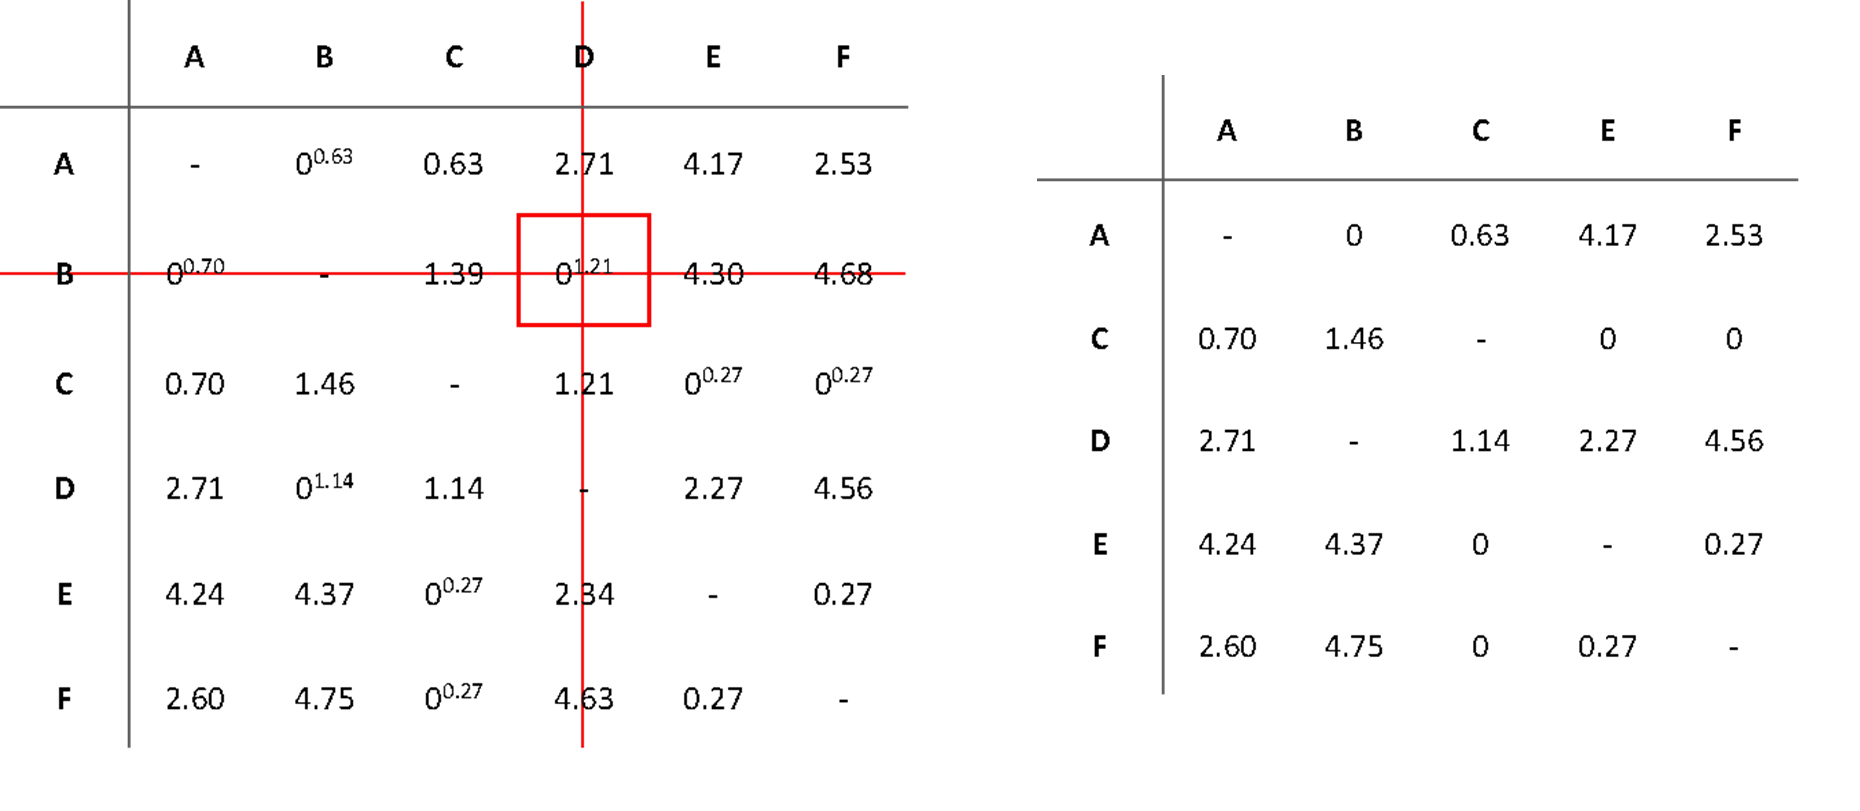
\includegraphics[height=6cm]{1elim2} 
\end{center}
	
\noindent
From this step we got a fraction of the final tour, namely road B $\rightarrow$ D, and a smaller matrix, for which we now repeat steps 1-3. Note that element DB is undefined, since road B $\rightarrow$ D is already taken.
	

\vspace{5mm}
\underline{Step 1}

\begin{center}
	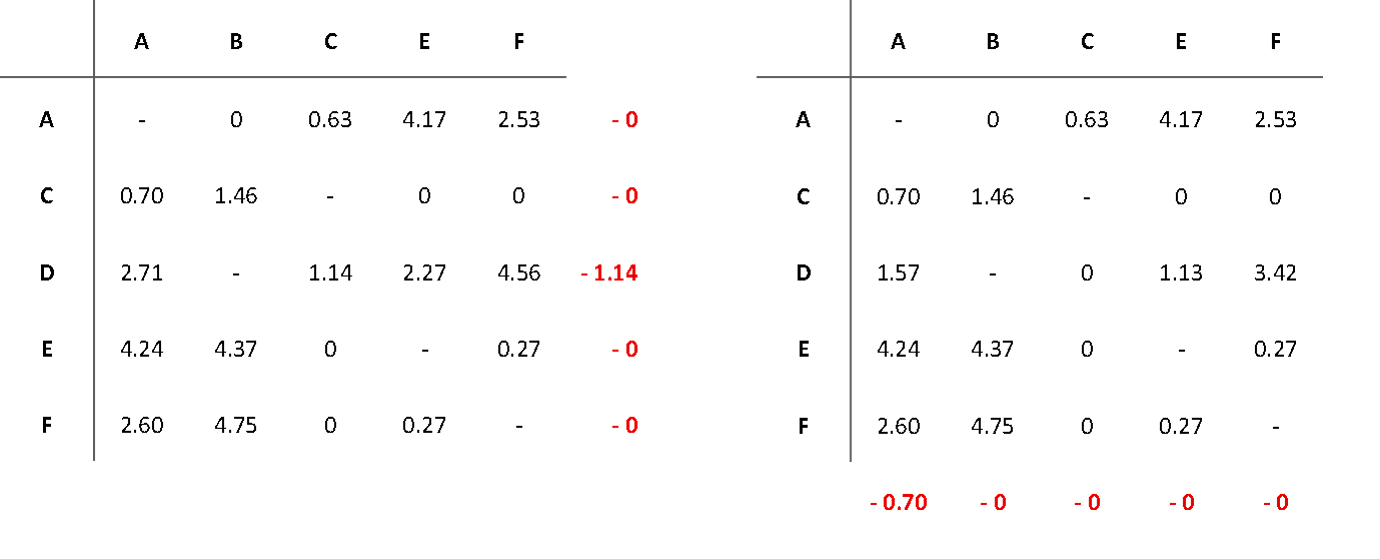
\includegraphics[height=5.6cm]{2red0} 
\end{center}	

\vspace{-3mm}
\underline{Step 2}

\begin{center}
	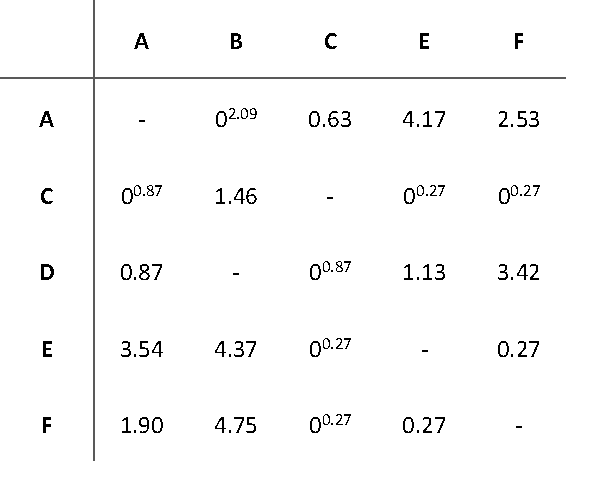
\includegraphics[height=5.2cm]{2pen}
\end{center}	
	
	
\underline{Step 3}

\begin{center}
	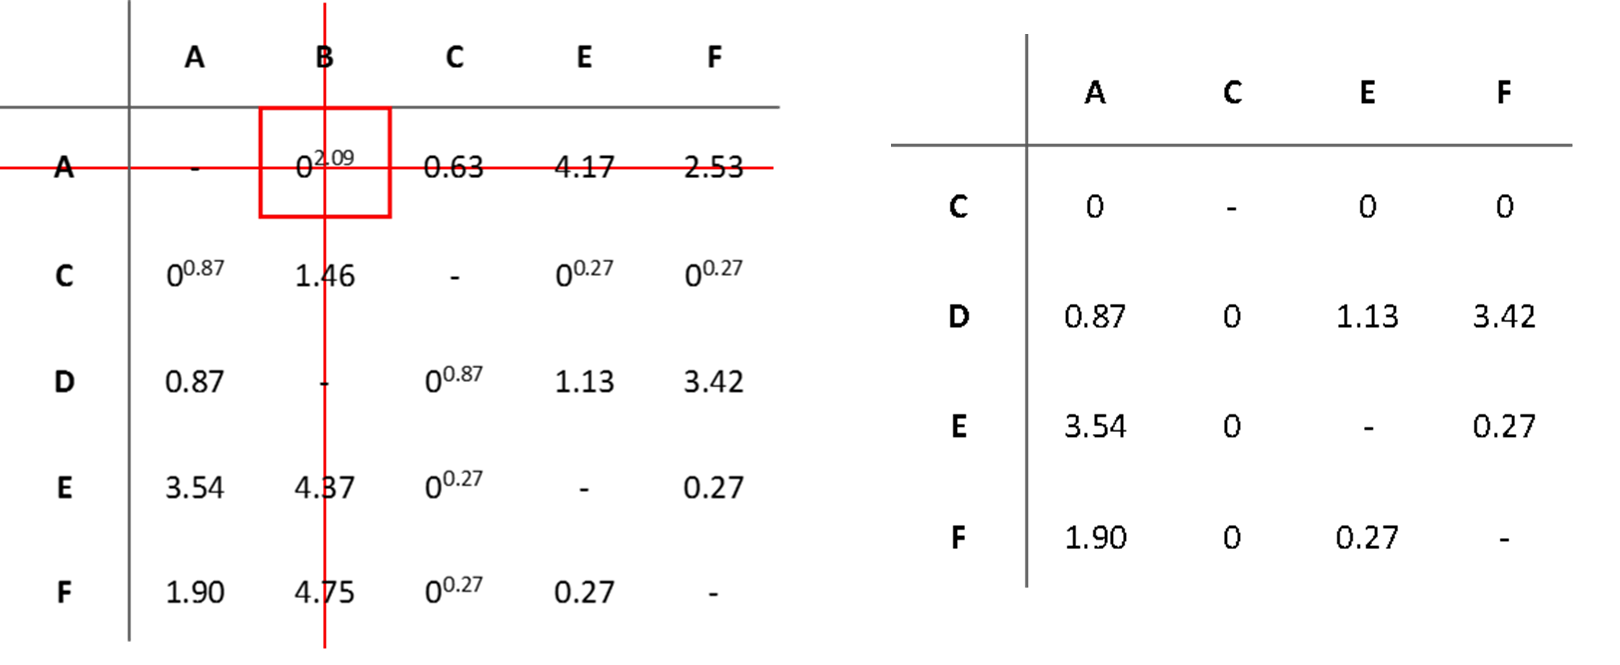
\includegraphics[height=5.2cm]{2elim3}
\end{center}

\noindent
Therefore, we add road A $\rightarrow$ B to the list and remove the value of element BA. In this case, row B has already been eliminated, so element BA already does not exist in the new matrix. Now repeat again. Notice that the newest matrix already contains a zero in every row and every column, so step 1 could be emitted.

\vspace{5mm}
\underline{Step 2}
\vspace{-3mm}
\begin{center}
	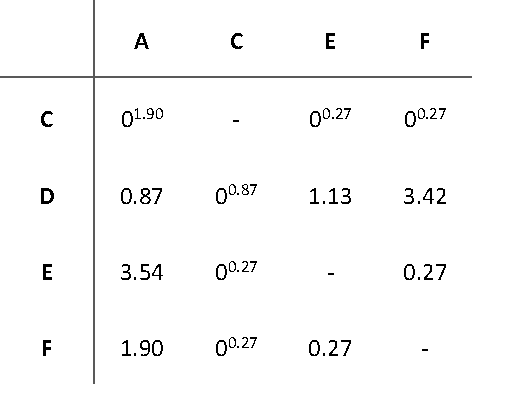
\includegraphics[height=4.8cm]{3pen}
\end{center}	

\underline{Step 3}
\vspace{-2mm}
\begin{center}
	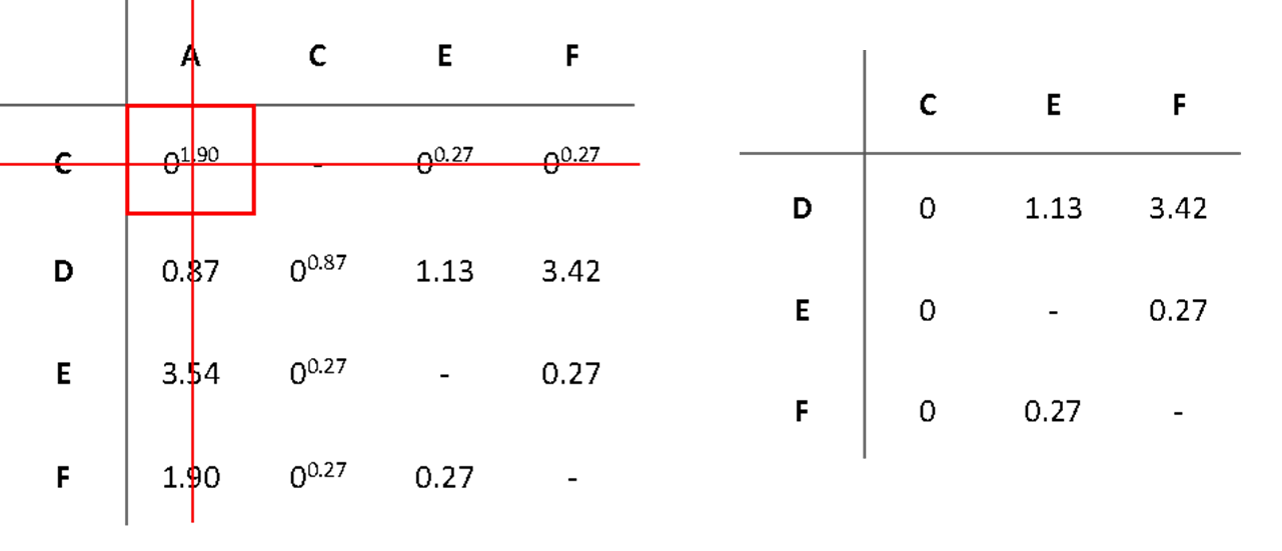
\includegraphics[height=4.5cm]{3elim4}
\end{center}

\noindent
Hence, we note down road C $\rightarrow$ A, and proceed with the 3x3 matrix.


\vspace{5mm}
\underline{Step 1} 

\begin{center}
	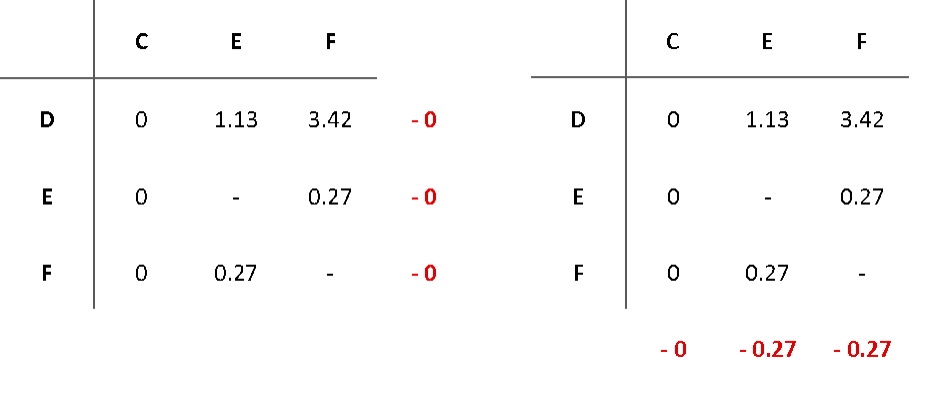
\includegraphics[height=4.2cm]{4red0} 
\end{center}	


\underline{Step 2} 
\vspace{-3mm}
\begin{center}
	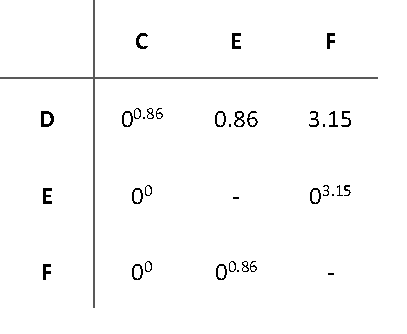
\includegraphics[height=3.7cm]{4pen}
\end{center}	


\underline{Step 3}
\vspace{-2mm}
\begin{center}
	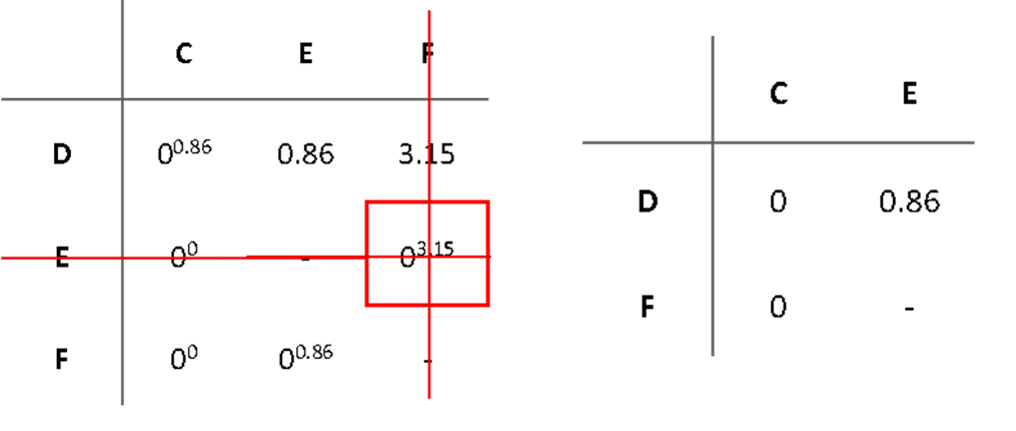
\includegraphics[height=3.6cm]{4elim5}
\end{center}

\noindent
Road E $\rightarrow$ F is now part of the tour, and element FE becomes undefined in the new 2x2 matrix. Now, one could proceed with the steps of the algorithm, but at this stage it is fairly simple to select the final tours: two are remaining and only two are possible: F~$\rightarrow$ C and D $\rightarrow$ E, which correspond to elements FC and DE respectively. DC cannot be selected because it would leave FE, which is not possible, so FC and DE is the correct choice.
Looking back, the following roads have been selected:
\begin{center}
	\par B $\rightarrow$ D, 
	\par A $\rightarrow$ B, 
	\par C $\rightarrow$ A, 
	\par E $\rightarrow$ F,
	\par F $\rightarrow$ C, 
	\par D $\rightarrow$ E.
\end{center}

\noindent
These roads can be compiled into a tour as follows:
\begin{center}
	A $\rightarrow$ B $\rightarrow$ D $\rightarrow$ E $\rightarrow$ F $\rightarrow$ C $\rightarrow$ A,
\end{center}
with city A chosen arbitrarily as the starting point. This completes the algorithm. 